% ============================================================================
%  Main document — wrapper for compiling the methodology section standalone
%
%  Compile with: pdflatex main.tex  (twice for references)
%  Or use:       latexmk -pdf main.tex
% ============================================================================
\documentclass[11pt, a4paper]{article}

% ── Geometry ──
\usepackage[margin=2.5cm]{geometry}

% ── Encoding & Fonts ──
\usepackage[utf8]{inputenc}
\usepackage[T1]{fontenc}
\usepackage{lmodern}

% ── Math ──
\usepackage{amsmath, amssymb, amsfonts}

% ── Graphics ──
\usepackage{graphicx}
\usepackage{xcolor}
\usepackage{subcaption}

% ── TikZ ──
\usepackage{tikz}
\usetikzlibrary{
    arrows.meta,
    positioning,
    shapes.geometric,
    shapes.misc,
    calc,
    fit,
    backgrounds,
    decorations.pathreplacing,
}

% ── Tables ──
\usepackage{booktabs}
\usepackage{multirow}

% ── Algorithms ──
\usepackage[ruled, vlined, linesnumbered]{algorithm2e}

% ── Hyperlinks ──
\usepackage[colorlinks=true, linkcolor=blue!60!black, citecolor=green!50!black, urlcolor=blue!70]{hyperref}

% ── CJK support (for character examples) ──
% Uncomment if CJK fonts are available on your system:
% \usepackage{CJKutf8}
% If CJK is not available, define a dummy environment:
\newenvironment{CJK}[3]{}{}

% ── Misc ──
\usepackage{microtype}


% ============================================================================
\title{Character Clustering from Historical Document Images:\\Methodology}
\author{}
\date{}

\begin{document}
\maketitle

% ============================================================================
%  Methodology Section — Historical Document Character Clustering Pipeline
% ============================================================================



% Stage I - Character extraction and recognition
% 
% a. CRAFT-based character detection, with dual-threshold watershed to extract connected components.
%
% b. Binarisation and association of connected components to CRAFT detections.
%
% c. Optical Character Recogntion
%    i) Layout analysis to determine columns, sub-columns and reading order
%    ii) Sub-column level OCR using a Kraken-based model trained on similar historical Chinese documents
%    iii) Spatial matching of OCR tokens to CRAFT detections via the Hungarian algorithm on vertical distances, to assign OCR labels to character patches. When no match is found, assign an unknown token.

%
% | Stage content:
%   - M1.1 / One page with the extracted character patches (example: outputs/extraction/book1/visualizations/characters/wdl_13516_033_segmentation.png)
%   - M1.2 / A zoom on one patch with connected components too large -> Cannot be used as a model (manual plot, should not be generated)
%   - M1.3 / CRAFT detection blobs, filtered by area, to show the points of the layout being falsely detected as characters (examplel: outputs/extraction/book1/visualizations/craft/wdl_13516_033_deletion.png)
%   - M1.4 / Layout analysis result, showing the detected columns and sub-columns
%   - M1.5 / OCR result, showing the predicted character sequence for one sub-column, and the spatial matching to CRAFT detections (plots that are in preprocessing_report.html)
%   - M1.6 / Alignment of the OCR results to the optional transcription (figure outputs/preprocessing/alignment_viz)
%
% Stage II - Preprocessing
%
% a. Rotation correction via LSD and length-weighted circular mean of line segment orientations
% b. Ink filter: area opening and closing to remove small holes and noise specks
% c. Vectorisation via affine scale-space smoothing, producing calligraphy-faithful SVG outlines
%
% | Stage content:
%   - M2.1 / Figure with (a) raw image patch, (b) binarised patch, and (c) clean, vectorised SVG outline with super resolution. This plot must show the recognized character as well.
%   - M2.2 / (perhaps the LSD result?)
% 
%
%
% Stage III - A contrario matching and graph-based clustering
%
% a. HOG descriptors computed on the vectorised character images (list all the parameters without specific values, which can be given in the experiments section)
% b. Pairwise dissimilarities computed using the Circular Earth Mover's Distance (CEMD) on the HOG descriptors
% c. A contrario framework to determine a statistically grounded matching threshold, computing the probability of a false alarm (NFA) for each pair of characters under a null model where dissimilarities are Gaussian
% d. Graph construction: vertices are character tokens, edges are created when both NLFA values exceed the threshold, and weighted by the symmetrised NLFA
% e. Correlation clustering via the Leiden algorithm to maximise the CPM quality function, sweeping over the NFA threshold and the resolution parameter to find the best clustering according to the Adjusted Rand Index. Prove the equivalence between CPM and LambdaCC, and justify the choice of CPM over modularity.
%
% | Stage content:
%   - M3.1 / Figure with (a) rendered vectorised character, (b) gradient magnitude, (c) gradient orientation, and (d) the resulting HOG descriptor (orientation bins $\times$ cell index).
%   - M3.2 / Figure with (a) histogram of pairwise dissimilarities for a query character and the fitted Gaussian null model, showing meaningful matches in the left tail; and (b) per-character null-model parameters across the corpus, with the query character marked.
%   - M3.3 / Examples of cluster before refinement (tsne_plot.py)
%
% Stage IV - Cluster refinement and glossary construction
%
% a. Cluster refinement via Hausdorff-based splitting
% b. Cluster refinement via OCR label splitting
%
% | Stage content:
%   - M4.1 / Character catalogue examples (manually generated)
%   - M4.2 / Glossary (old fig. 13, split in three parts: 4 rows for the most frequent clusters, 4 rows for the characters whose max cluster size is two, 4 rows for the least)
%   - M4.3 / Reverse printed manuscript (already generated)
%
% | Also:
%   - ARI etc. vs Hausdorff threshold
%   - Discrepancy statistics
%   - ...


% 3. Character vectorisation
%   We use affine scale-space smoothing, an affine-invariant geometric PDE that evolves each level line according to its curvature, producing smooth vector outlines.
%   Document skew is estimated using LSD and corrected via the length-weighted circular mean of line segment orientations.
%   Additionally, we apply a small filter (what is it's name already?) to clean the binary patches before vectorisation, removing small holes and noise specks.
% 4. Glyph extraction
%   So far, we have:
%   - a set of (possibly noisy) vectorized character images
%   - an OCR label
%   We wish to get the best possible character image for each character in the book.
%   Intuitively, this character should be the most similar to the other instances of the same character.
%
%   Steps for the extraction:
%    a. Compute HOG descriptors on the vectorised character images (rendered at 256 DPI, 24x24 px cells, 16 bins per cell, Gaussian derivative filters with sigma=5 and kernel size=31 px, L2-clip-L2 normalisation with clipping threshold t=0.2).
%    b. Compute pairwise dissimilarities using the Circular Earth Mover's Distance (CEMD) on the HOG descriptors.
%    c. Use an a contrario framework to determine a statistically grounded matching threshold, computing the probability of a false alarm (NFA) for each pair of characters under a null model where dissimilarities are Gaussian
%    d. Construct a graph weighted by the NFA scores and partition it using the Leiden algorithm, to minimise the correlation clustering disagreement objective (x).
%       We sweep over the NFA threshold and the resolution parameter of the Leiden algorithm to find the best clustering according to the Adjusted Rand Index (ARI) with respect to the OCR labels.
%    e. Refine the clusters via a three-stage process:
%       1. Large clusters (>=5 members) are split using hierarchical clustering on pairwise Hausdorff distances computed on registered binary images (registration via multiscale inverse compositional alignment
%       2. Split the clusters by OCR label
%    The new clusters are:
%       1. Guaranteed to be pure according to the OCR
%       2. Guaranteed to be more compact in terms of Hausdorff distance (criterion: average linkage dendrogram cut at tau_split=21.5)
%    Therefore, in the biggest cluster, the most representative character is likely to be a good candidate for the glossary.
%    When the two biggest clusters have the same size, we use the intra NFA as a tie-breaker, selecting the cluster with the lowest mean intra-cluster NFA.
%    Criterions for the representative:
%       a - the character that minimises the mean intra-cluster dissimilarity.
%       b - the most central according to the degree or weighted degree in the similarity graph.
%       c - ...


% Figures:
% - Overview of character extraction, layout analysis, OCR transcription, transcription matching and OCR/transcription match.
% - Preprocessing result - ie. why vectorisation and ink filter are necessary, showing the raw binary patch and the resulting vector outline with super resolution
% - An example of the HOG descriptor, showing the rendered character, the gradient field and the resulting histogram.
% - Distribution test for the a contrario model, showing the histogram of dissimilarities and the fitted Gaussian.
% - One cluster, before and after refinement
% - The final glossary, showing the representative character for each cluster along with its frequency and OCR label.

\section{Methodology}
\label{sec:methodology}

Our pipeline processes scanned historical document images to produce a vectorised character glossary through four stages: (1)~character extraction and recognition, (2)~preprocessing, (3)~\textit{a contrario} matching and graph-based clustering, and (4)~cluster refinement, glossary construction, and reverse printing.
Figure~\ref{fig:pipeline-overview} presents an overview.

% ============================================================================
%  Pipeline Overview Figure — full-page flowchart
% ============================================================================
\begin{figure}[t]
    \centering
    \resizebox{0.65\linewidth}{!}{%
    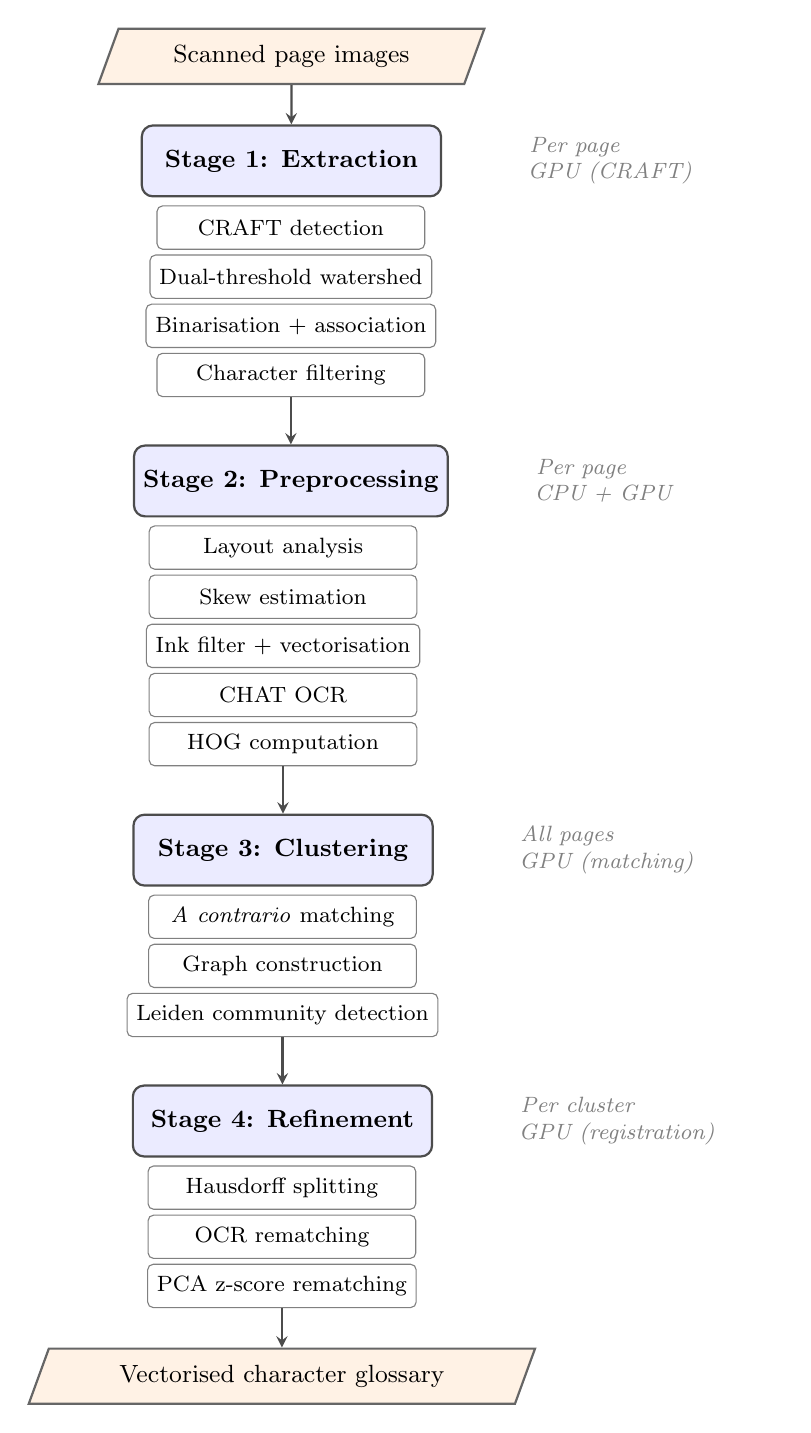
\begin{tikzpicture}[
        >=stealth,
        node distance=0.4cm and 1.0cm,
        stage/.style={
            rectangle, rounded corners=4pt, draw=black!70, thick,
            fill=blue!8, minimum width=3.8cm, minimum height=0.9cm,
            text centered, font=\small\bfseries
        },
        substage/.style={
            rectangle, rounded corners=2pt, draw=black!50,
            fill=white, minimum width=3.4cm, minimum height=0.55cm,
            text centered, font=\footnotesize
        },
        io/.style={
            trapezium, trapezium left angle=70, trapezium right angle=110,
            draw=black!60, fill=orange!10, thick,
            minimum width=2.8cm, minimum height=0.7cm,
            text centered, font=\small
        },
        arrow/.style={->, thick, black!70},
        darrow/.style={->, thick, black!70, dashed},
        group/.style={
            draw=gray!50, dashed, rounded corners=6pt, inner sep=8pt
        },
    ]

    % ── Input ──
    \node[io] (input) {Scanned page images};

    % ── Stage 1: Extraction ──
    \node[stage, below=0.5cm of input] (extraction) {Stage 1: Extraction};
    \node[substage, below=0.1cm of extraction.south west, anchor=north west, xshift=0.2cm]
        (craft) {CRAFT detection};
    \node[substage, below=0.06cm of craft]
        (watershed) {Dual-threshold watershed};
    \node[substage, below=0.06cm of watershed]
        (binarise) {Binarisation + association};
    \node[substage, below=0.06cm of binarise]
        (charfilter) {Character filtering};

    % ── Stage 2: Preprocessing ──
    \node[stage, below=0.6cm of charfilter] (preproc) {Stage 2: Preprocessing};
    \node[substage, below=0.1cm of preproc.south west, anchor=north west, xshift=0.2cm]
        (layout) {Layout analysis};
    \node[substage, below=0.06cm of layout]
        (skew) {Skew estimation};
    \node[substage, below=0.06cm of skew]
        (inkfilt) {Ink filter + vectorisation};
    \node[substage, below=0.06cm of inkfilt]
        (chatocr) {CHAT OCR};
    \node[substage, below=0.06cm of chatocr]
        (hogcomp) {HOG computation};

    % ── Stage 3: Clustering ──
    \node[stage, below=0.6cm of hogcomp] (cluster) {Stage 3: Clustering};
    \node[substage, below=0.1cm of cluster.south west, anchor=north west, xshift=0.2cm]
        (acontrario) {\textit{A contrario} matching};
    \node[substage, below=0.06cm of acontrario]
        (graph) {Graph construction};
    \node[substage, below=0.06cm of graph]
        (leiden) {Leiden community detection};

    % ── Stage 4: Refinement ──
    \node[stage, below=0.6cm of leiden] (refine) {Stage 4: Refinement};
    \node[substage, below=0.1cm of refine.south west, anchor=north west, xshift=0.2cm]
        (hausdorff) {Hausdorff splitting};
    \node[substage, below=0.06cm of hausdorff]
        (ocrrematch) {OCR rematching};
    \node[substage, below=0.06cm of ocrrematch]
        (pcarematch) {PCA z-score rematching};

    % ── Output ──
    \node[io, below=0.5cm of pcarematch] (output) {Vectorised character glossary};

    % ── Arrows ──
    \draw[arrow] (input) -- (extraction);
    \draw[arrow] (charfilter.south) -- ++(0,-0.2) -| (preproc);
    \draw[arrow] (hogcomp.south) -- ++(0,-0.2) -| (cluster);
    \draw[arrow] (leiden.south) -- ++(0,-0.2) -| (refine);
    \draw[arrow] (pcarematch.south) -- ++(0,-0.2) -| (output);

    % ── Side annotations ──
    \node[right=1.0cm of extraction, text=gray, font=\footnotesize\itshape, text width=3cm]
        {Per page\\GPU (CRAFT)};
    \node[right=1.0cm of preproc, text=gray, font=\footnotesize\itshape, text width=3cm]
        {Per page\\CPU + GPU};
    \node[right=1.0cm of cluster, text=gray, font=\footnotesize\itshape, text width=3cm]
        {All pages\\GPU (matching)};
    \node[right=1.0cm of refine, text=gray, font=\footnotesize\itshape, text width=3cm]
        {Per cluster\\GPU (registration)};

    \end{tikzpicture}%
    }
    \caption{Overview of the reverse typography pipeline.
    Scanned page images are processed through four sequential stages to produce a vectorised character glossary.
    Stages are annotated with their computational scope (per-page vs.\ global) and primary hardware usage.}
    \label{fig:pipeline-overview}
\end{figure}



% ============================================================================
\subsection{Character Extraction and Recognition}
\label{sec:extraction}

This stage takes a scanned page image and produces, for each detected character, a binary image, a bounding box, and an OCR-predicted label.

% ── (a) CRAFT-based character detection ──
\paragraph{CRAFT-based character detection.}
We use CRAFT~\cite{baek2019character} (\textit{Character Region Awareness for Text Detection}), a fully convolutional network producing per-pixel text score maps $S_\text{text}(x, y) \in [0,1]$.
We use pre-trained weights without fine-tuning, with magnification ratio~$5.0$ (canvas size 1280\,px).

Connected components are extracted via dual-threshold watershed: pixels with $S_\text{text} \ge \tau_\text{text} = 0.6$ serve as seeds, and basins expand to a lower mask threshold $\tau_\text{mask} = 0.3$.
Components with area below 10\,px are discarded as noise (area opening).

% ── (b) Binarisation and component association ──
\paragraph{Binarisation and component association.}
In parallel, the page is binarised (Otsu's method) and binary connected components are associated with CRAFT detections via negative Mahalanobis distance using each CRAFT region's inertia tensor.
Each binary component is assigned to the CRAFT detection whose elliptic distance is smallest, yielding a set of character candidates with both a binary image and a precise bounding box.
Filters discard components outside the expected bounding-box range ($30 \times 30$ to $250 \times 250$\,px) or with insufficient filled area ($<700$\,px$^2$).

% ── M1.1: Extraction segmentation figure ──
\begin{figure}[t]
    \centering
    \includegraphics[width=\linewidth]{\figExtractionSeg}
    \caption{Character extraction result on a representative page.
    Bounding boxes show the final character candidates after CRAFT detection,
    watershed segmentation, Mahalanobis association, and post-filtering.
    Colour coding indicates deletion reasons for discarded components.}
    \label{fig:extraction-segmentation}
\end{figure}

% ── M1.3: CRAFT deletion reasons figure ──
\begin{figure}[t]
    \centering
    \includegraphics[width=\linewidth]{\figCraftDeletion}
    \caption{CRAFT detection with deletion-reason overlay.
    Components that pass all filters are shown in green; discarded
    components are colour-coded by rejection criterion (red~=~area too
    small, orange~=~aspect ratio too low, purple~=~high aspect ratio,
    pink~=~box too small, magenta~=~box too large, blue~=~too close to
    page contour).}
    \label{fig:craft-deletion}
\end{figure}

% ── (c) Optical character recognition ──
\paragraph{Layout analysis and reading order.}
A projection-based layout module identifies columns and sub-columns from vertical ink-density profiles.
Columns are detected by computing horizontal projections on the binarised image and thresholding the resulting profile.
Within each column, rows are segmented using vertical projections, and further subdivision into sub-columns handles cases where multiple text lanes coexist within a single column.
The reading order follows the right-to-left, top-to-bottom convention of classical Chinese, assigning each character an integer index.
Figure~\ref{fig:layout-analysis} illustrates the column and sub-column detection on a representative page.

% ── M1.4: Layout analysis figure ──
\begin{figure}[t]
    \centering
    \includegraphics[width=\linewidth]{\figLayoutAnalysis}
    \caption{Layout analysis result showing column and sub-column detection.
    \emph{Top:} horizontal ink-density projection with detected column
    boundaries.
    \emph{Bottom:} page image with column overlays (distinct colours) and
    sub-column boundaries (dashed lines within each column).
    The reading order proceeds right-to-left across columns and
    top-to-bottom within each sub-column.}
    \label{fig:layout-analysis}
\end{figure}

\paragraph{Character recognition.}
Characters are labelled using a Kraken-based~\cite{kiessling2019kraken} model trained on similar historical Chinese documents, operating at the sub-column level.
A baseline is extracted by taking the median of the $x$-barycenters of the characters within each sub-column.
Predicted character sequences are spatially matched to CRAFT detections via the Hungarian algorithm on vertical distances.
When no detection can be matched, the character is assigned an unknown token~$\square$.
Each character receives a label $\ell_i \in \mathcal{A} \cup \{\square\}$.

When an external transcription is available, it is aligned to the OCR predictions using Levenshtein edit distance, yielding a ground-truth label for each patch (Section~\ref{sec:eval-protocol}).


% ============================================================================
\subsection{Preprocessing}
\label{sec:preprocessing}

Each extracted character patch undergoes rotation correction, morphological cleaning, and vectorisation to produce a resolution-independent SVG outline faithful to the original calligraphy.
Figure~\ref{fig:preprocessing} illustrates the three stages on representative examples.

% ── M2.1: Preprocessing before/after figure ──
\begin{figure}[t]
    \centering
    \includegraphics[width=\linewidth]{\figPreprocessing}
    \caption{Preprocessing pipeline for individual character patches.
    \emph{Top row:} raw image patches extracted by CRAFT.
    \emph{Middle row:} binarised patches after Otsu thresholding and morphological cleaning.
    \emph{Bottom row:} vectorised SVG outlines produced by affine scale-space smoothing.}
    \label{fig:preprocessing}
\end{figure}

% ── (a) Rotation correction ──
\paragraph{Rotation correction.}
Document skew is estimated using LSD~\cite{von2010lsd} (\textit{Line Segment Detector}).
Dominant line segment orientations are aggregated via a length-weighted circular mean:
\begin{equation}
    \theta = \tfrac{1}{2}\arg\!\left(\textstyle\sum_i w_i \, e^{2\mathrm{i}\alpha_i}\right),
    \label{eq:skew}
\end{equation}
where $w_i$ and $\alpha_i$ are the length and orientation of each detected line segment.
The estimated angle $\theta$ is applied as a global rotation correction to each character patch.

% ── (b) Ink filter ──
\paragraph{Ink filter.}
Binary patches are cleaned by area opening and area closing (removing foreground specks below 5\,px and background holes below 10\,px), producing a crisp binary image suitable for vectorisation.

% ── (c) Vectorisation via affine scale-space ──
\paragraph{Vectorisation via affine scale-space.}
Cleaned binary patches are vectorised using affine scale-space smoothing~\cite{alvarez1993axioms,ciomaga2017curvature}.
This geometric PDE evolves each level line of the image according to its curvature:
\begin{equation}
    \frac{\partial u}{\partial t} = |\nabla u|\, \kappa^{1/3},
    \label{eq:gass}
\end{equation}
where $\kappa$ denotes the curvature of the level line through each point.
The $1/3$ exponent makes this evolution affine-invariant: the smoothed shape is independent of the viewing angle, which is essential for comparing characters printed under different conditions.
The resulting smooth level lines are converted to SVG vector outlines, yielding a calligraphy-faithful, resolution-independent representation of each character.


% ============================================================================
\subsection{A Contrario Matching and Clustering}
\label{sec:acontrario}

This stage computes a visual descriptor for each character, assesses pairwise similarity using a statistical framework, and partitions the characters into clusters.

% ── (a) HOG descriptors ──
\paragraph{HOG descriptors.}
Each character is described by a Histogram of Oriented Gradients (HOG) descriptor~\cite{dalal2005histograms} computed on a rendered SVG image.
The character is rasterised at a fixed resolution into a grid of $C \times C$ cells.
Gradients are computed using Gaussian derivative filters with smoothing parameter~$\sigma$ and accumulated into $B$ unsigned orientation bins per cell via trilinear interpolation:
\begin{equation}
    h_b = \sum_{(x,y) \in \text{cell}} m(x,y) \cdot \bigl[(1 - \alpha)\,\delta_{b, \lfloor \hat\theta \rfloor} + \alpha\,\delta_{b, (\lfloor \hat\theta \rfloor + 1) \bmod B}\bigr],
\end{equation}
where $\hat\theta = \theta \cdot B$ and $\alpha = \hat\theta - \lfloor\hat\theta\rfloor$.
The descriptor is normalised via L2-clip-L2 with clipping threshold~$t$.
Specific parameter values are reported in Section~\ref{sec:experiments}.

% ============================================================================
%  HOG Descriptor Computation Figure
% ============================================================================
\begin{figure}[t]
    \centering
    \resizebox{\linewidth}{!}{%
    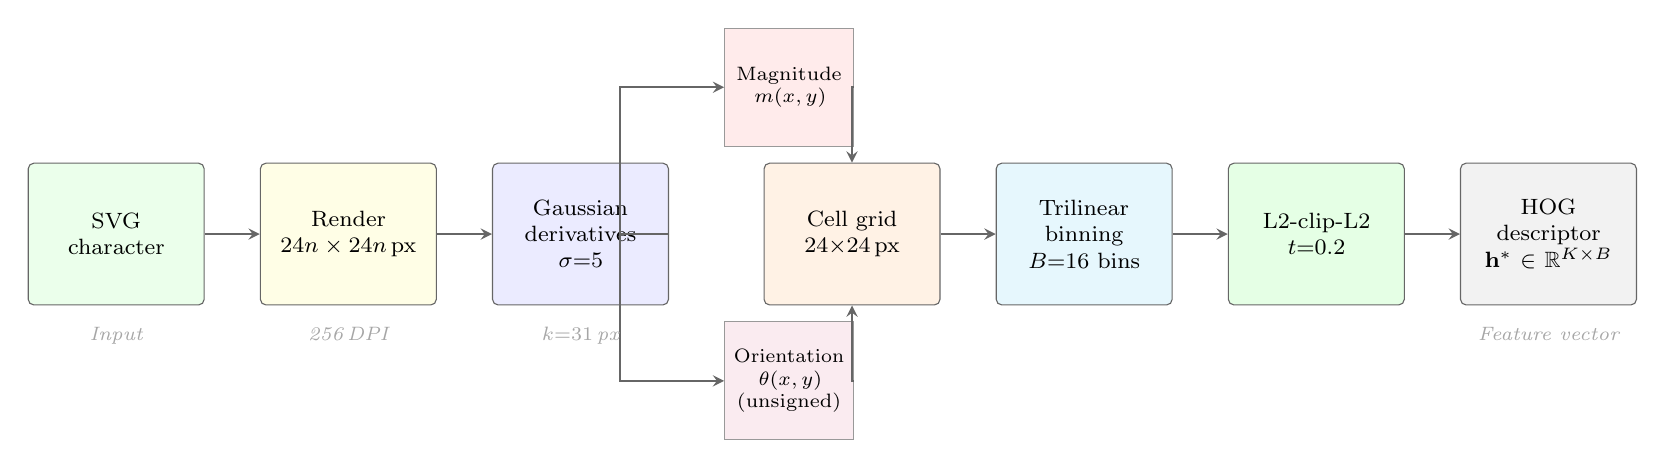
\begin{tikzpicture}[
        >=stealth,
        node distance=0.5cm and 0.8cm,
        box/.style={
            rectangle, rounded corners=2pt, draw=black!60,
            fill=#1, minimum width=2.2cm, minimum height=1.8cm,
            text centered, font=\footnotesize, text width=2cm
        },
        box/.default=white,
        smallbox/.style={
            rectangle, draw=black!40, fill=#1,
            minimum width=1.5cm, minimum height=1.5cm,
            text centered, font=\scriptsize, text width=1.4cm
        },
        smallbox/.default=white,
        arrow/.style={->, thick, black!60},
        label/.style={font=\scriptsize\itshape, text=gray!70},
    ]

    % ── SVG input ──
    \node[box=green!8] (svg) {SVG\\character};

    % ── Render ──
    \node[box=yellow!10, right=0.7cm of svg] (render) {Render\\$24n \times 24n$\,px};

    % ── Gaussian derivative ──
    \node[box=blue!8, right=0.7cm of render] (gradient) {Gaussian\\derivatives\\$\sigma{=}5$};

    % ── Magnitude + Orientation ──
    \node[smallbox=red!8, above right=0.2cm and 0.7cm of gradient] (magn)
        {Magnitude\\$m(x,y)$};
    \node[smallbox=purple!8, below right=0.2cm and 0.7cm of gradient] (orient)
        {Orientation\\$\theta(x,y)$\\(unsigned)};

    % ── Cell decomposition ──
    \node[box=orange!10, right=1.2cm of gradient, yshift=0cm] (cells)
        {Cell grid\\$24{\times}24$\,px};

    % ── Histogram ──
    \node[box=cyan!10, right=0.7cm of cells] (hist)
        {Trilinear\\binning\\$B{=}16$ bins};

    % ── Normalize ──
    \node[box=green!10, right=0.7cm of hist] (norm)
        {L2-clip-L2\\$t{=}0.2$};

    % ── Output ──
    \node[box=gray!10, right=0.7cm of norm] (output)
        {HOG\\descriptor\\$\mathbf{h}^* \in \mathbb{R}^{K \times B}$};

    % ── Arrows ──
    \draw[arrow] (svg) -- (render);
    \draw[arrow] (render) -- (gradient);
    \draw[arrow] (gradient) -- ++(0.5, 0) |- (magn);
    \draw[arrow] (gradient) -- ++(0.5, 0) |- (orient);
    \draw[arrow] (magn) -| (cells);
    \draw[arrow] (orient) -| (cells);
    \draw[arrow] (cells) -- (hist);
    \draw[arrow] (hist) -- (norm);
    \draw[arrow] (norm) -- (output);

    % ── Labels below ──
    \node[label, below=0.15cm of svg] {Input};
    \node[label, below=0.15cm of render] {256\,DPI};
    \node[label, below=0.15cm of gradient] {$k{=}31$\,px};
    \node[label, below=0.15cm of output] {Feature vector};

    \end{tikzpicture}%
    }
    \caption{HOG descriptor computation pipeline.
    Each character's SVG is rendered onto a pixel grid, smoothed with Gaussian derivative filters, decomposed into cells, and each cell's gradient histogram is computed via trilinear interpolation.
    The concatenated histograms are normalised using L2-clip-L2 to produce the final descriptor.}
    \label{fig:hog-pipeline}
\end{figure}


% ── M3.1: HOG descriptor example figure ──
\begin{figure}[t]
    \centering
    \includegraphics[width=\linewidth]{\figHogDescriptor}
    \caption{HOG descriptor computation on a representative character.
    From left to right: rendered SVG, gradient magnitude, gradient orientation, and the resulting HOG descriptor (orientation bins $\times$ cell index).}
    \label{fig:hog-example}
\end{figure}

% ── (b) Dissimilarity metric ──
\paragraph{Dissimilarity metric.}
Given two HOG descriptors $\mathbf{h}^A, \mathbf{h}^B$ with $K$ cells of $B$ bins each, we compute the Circular Earth Mover's Distance (CEMD) per cell.
For cumulative difference $X_j = \sum_{i=1}^{j} h^A_{k,i} - \sum_{i=1}^{j} h^B_{k,i}$:
\begin{equation}
    \text{CEMD}(h^A_k, h^B_k) = \min_{s \in \{0,\ldots,B{-}2\}} \frac{1}{B}\sum_{j=1}^{B} |X_j - X_s|.
    \label{eq:cemd}
\end{equation}
The total dissimilarity is $D(\mathbf{h}^A, \mathbf{h}^B) = \sum_{k=1}^{K} \text{CEMD}(h^A_k, h^B_k)$.

% ── (c) Number of False Alarms ──
\paragraph{Number of False Alarms.}
Character similarity is assessed using an \textit{a contrario} framework~\cite{desolneux2000meaningful} that provides a statistically grounded matching threshold.
Under the null model, $D$ is approximately Gaussian with character-specific moments $(\mu_A, \sigma_A^2)$ estimated from all pairwise comparisons.
The NFA is:
\begin{equation}
    \text{NFA}(A,B) = N^2 \cdot \Phi\!\left(\frac{D(\mathbf{h}^A, \mathbf{h}^B) - \mu_A}{\sigma_A}\right),
    \label{eq:nfa}
\end{equation}
where $\Phi$ is the standard normal CDF.
Two characters are meaningfully similar when $\text{NFA} \le \varepsilon$.
We store the negative log-NFA: $\text{NLFA}(A,B) = -\log\Phi\!\bigl(\frac{D - \mu_A}{\sigma_A}\bigr)$.

% ── M3.2: A contrario distribution figure ──
\begin{figure}[t]
    \centering
    \includegraphics[width=\linewidth]{\figAContrario}
    \caption{A contrario null-hypothesis test.
    \emph{Left:} histogram of pairwise dissimilarities for a query character and the fitted Gaussian null model $\mathcal{N}(\mu_A, \sigma_A^2)$.
    Characters with dissimilarity in the far left tail are \emph{meaningful} matches.
    \emph{Right:} per-character null-model parameters $(\mu_i, \sigma_i)$ across the corpus; the query character is marked in red.}
    \label{fig:a-contrario}
\end{figure}

% ── (d) Graph construction ──
\paragraph{Similarity graph.}
A graph $G = (V, E, w)$ is built with one vertex per character token.
An edge $(i,j)$ is created when both NLFA values exceed threshold $\tau_\text{NFA} = -\log\varepsilon + 2\log N$:
\begin{equation}
    (i,j) \in E \iff \text{NLFA}(i,j) \ge \tau_\text{NFA} \;\wedge\; \text{NLFA}(j,i) \ge \tau_\text{NFA}.
    \label{eq:reciprocal}
\end{equation}
The reciprocal condition discards asymmetric similarities.
Edge weights are the symmetrised NLFA: $w_{ij} = \tfrac{1}{2}[\text{NLFA}(i,j) + \text{NLFA}(j,i)]$.

% ── (e) Correlation clustering ──
\paragraph{Problem formulation.}
We seek a partition of the $N$ character tokens into clusters, one per distinct character.
The NFA scores $p_{ij}$ are ordinal---they rank pairs by similarity but are not calibrated probabilities---the number of distinct characters is unknown (though a lower bound is available from the OCR vocabulary), and the cluster size distribution is expected to follow a Zipf law: a few high-frequency characters and many rare ones.

We cast this as a \emph{correlation clustering} problem~\cite{bansal2004correlation}: given a graph where tokens are nodes and edges encode pairwise similarity, find a partition minimising the total \emph{disagreement}---the cost of placing dissimilar tokens together plus the cost of separating similar tokens.

\paragraph{CPM objective.}
For an unweighted-node correlation clustering problem with resolution $\gamma \in (0,1)$, the \emph{LambdaCC} disagreement objective~\cite{veldt2018correlation} is:
\begin{equation}
    \mathcal{L}_\gamma(\mathcal{C}) = \!\sum_{(i,j)\in E}\!(1{-}\gamma)\, x_{ij}
        + \!\sum_{(i,j)\notin E}\!\gamma\,(1{-}x_{ij}),
    \label{eq:lambdacc}
\end{equation}
where $x_{ij} = 0$ if $i,j$ are co-clustered and $1$ otherwise.
Expanding in terms of within-cluster edge weight $e_c$ and cluster size $n_c$ shows that $\mathcal{L}_\gamma = \text{const} - \mathcal{Q}_\gamma$, where
\begin{equation}
    \mathcal{Q}_\gamma = \sum_{c} \left[e_c - \gamma \binom{n_c}{2}\right]
    \label{eq:cpm}
\end{equation}
is the Constant Potts Model (CPM) quality function~\cite{traag2011narrow}.
Minimising disagreement is thus equivalent to maximising $\mathcal{Q}_\gamma$.

The CPM is a special case of the Reichardt--Bornholdt framework~\cite{reichardt2006statistical} with an Erd\H{o}s--R\'enyi null model ($P_{ij} = \text{const}$), in contrast to the configuration-model null model that yields modularity.
CPM is preferred here for three reasons:
\begin{enumerate}[nosep]
    \item \emph{No resolution limit.}  Modularity cannot resolve clusters smaller than ${\sim}\sqrt{2m}$ edges~\cite{fortunato2007resolution}, which would merge rare characters.  CPM has no such limitation.
    \item \emph{Ordinal compatibility.}  Only the relative ordering of edge weights matters, not their absolute calibration---appropriate for NFA-derived scores.
    \item \emph{Density interpretation.}  The resolution parameter $\gamma$ has a direct meaning: every cluster in an optimal partition has internal edge density $\ge \gamma$.
\end{enumerate}

\paragraph{Optimisation.}
We optimise $\mathcal{Q}_\gamma$ using the Leiden algorithm~\cite{traag2019louvain}, which guarantees well-connected communities and runs in seconds at our scale (${\sim}$\nNodes{} tokens, ${\sim}$\nEdges{} edges).
We sweep over both $\varepsilon$ and $\gamma$, selecting the configuration maximising ARI with respect to OCR labels (Section~\ref{sec:sensitivity}).

% ============================================================================
%  Clustering Pipeline Figure — a contrario matching → graph → Leiden
% ============================================================================
\begin{figure}[t]
    \centering
    \resizebox{\linewidth}{!}{%
    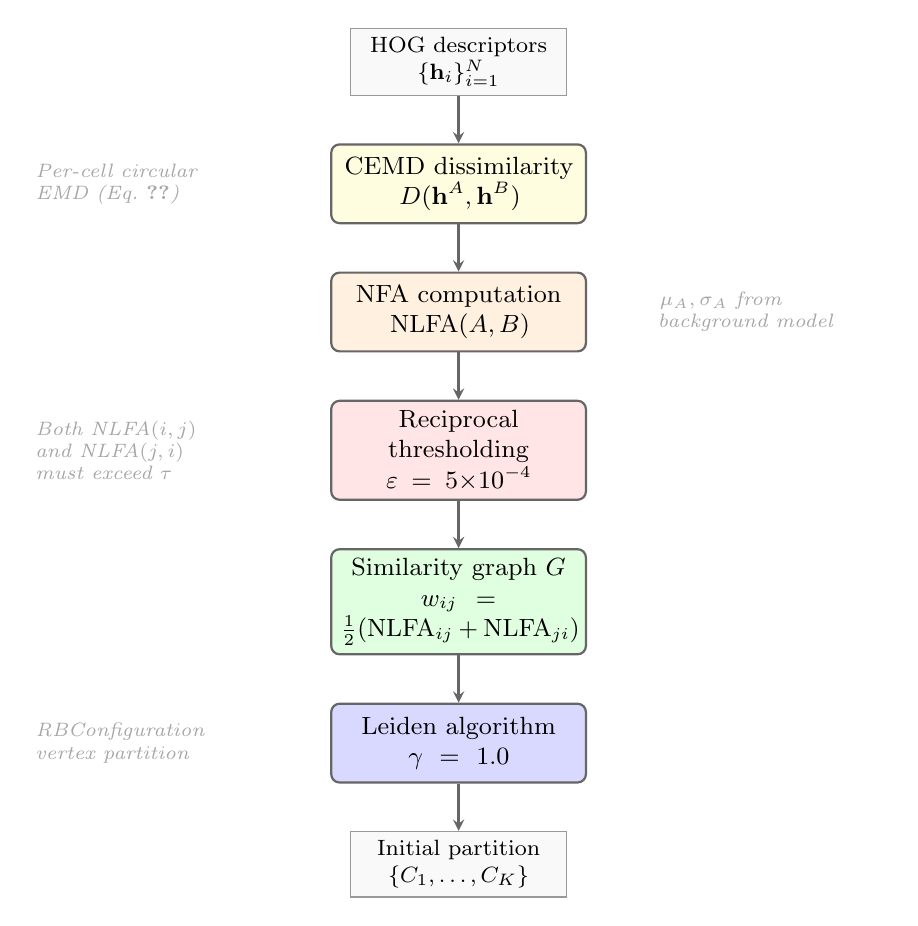
\begin{tikzpicture}[
        >=stealth,
        node distance=0.4cm and 1.0cm,
        process/.style={
            rectangle, rounded corners=3pt, draw=black!60, thick,
            fill=#1, minimum width=3.2cm, minimum height=1.0cm,
            text centered, font=\small, text width=3cm
        },
        process/.default=blue!8,
        data/.style={
            rectangle, draw=black!40, fill=gray!5,
            minimum width=2.6cm, minimum height=0.7cm,
            text centered, font=\footnotesize, text width=2.5cm
        },
        arrow/.style={->, thick, black!60},
        note/.style={font=\scriptsize\itshape, text=gray!70, text width=2.8cm},
    ]

    % ── Row 1: HOG features ──
    \node[data] (hog) {HOG descriptors\\$\{\mathbf{h}_i\}_{i=1}^N$};

    % ── Row 2: Dissimilarity ──
    \node[process=yellow!12, below=0.6cm of hog] (dissim)
        {CEMD dissimilarity\\$D(\mathbf{h}^A, \mathbf{h}^B)$};

    % ── Row 3: NFA ──
    \node[process=orange!12, below=0.6cm of dissim] (nfa)
        {NFA computation\\$\text{NLFA}(A,B)$};
    \node[note, right=0.8cm of nfa] {$\mu_A, \sigma_A$ from\\background model};

    % ── Row 4: Thresholding ──
    \node[process=red!10, below=0.6cm of nfa] (threshold)
        {Reciprocal thresholding\\$\varepsilon = 5{\times}10^{-4}$};

    % ── Row 5: Graph ──
    \node[process=green!12, below=0.6cm of threshold] (graph)
        {Similarity graph $G$\\$w_{ij} = \frac{1}{2}(\text{NLFA}_{ij} + \text{NLFA}_{ji})$};

    % ── Row 6: Leiden ──
    \node[process=blue!15, below=0.6cm of graph] (leiden)
        {Leiden algorithm\\$\gamma = 1.0$};

    % ── Row 7: Output ──
    \node[data, below=0.6cm of leiden] (partition)
        {Initial partition\\$\{C_1, \ldots, C_K\}$};

    % ── Arrows ──
    \draw[arrow] (hog) -- (dissim);
    \draw[arrow] (dissim) -- (nfa);
    \draw[arrow] (nfa) -- (threshold);
    \draw[arrow] (threshold) -- (graph);
    \draw[arrow] (graph) -- (leiden);
    \draw[arrow] (leiden) -- (partition);

    % ── Side annotations ──
    \node[note, left=0.8cm of dissim] {Per-cell circular\\EMD (Eq.~\ref{eq:cemd})};
    \node[note, left=0.8cm of threshold] {Both $\text{NLFA}(i,j)$\\and $\text{NLFA}(j,i)$\\must exceed $\tau$};
    \node[note, left=0.8cm of leiden] {RBConfiguration\\vertex partition};

    \end{tikzpicture}%
    }
    \caption{Clustering pipeline: from HOG features to an initial partition.
    Pairwise CEMD dissimilarities are converted into NFA scores under the \textit{a contrario} model, thresholded reciprocally to build a similarity graph, and partitioned by the Leiden algorithm.}
    \label{fig:clustering-pipeline}
\end{figure}



% ============================================================================
\subsection{Cluster Refinement, Glossary Construction, and Reverse Printing}
\label{sec:refinement}

The Leiden partition may contain impure or over-fragmented clusters.
A sequential two-stage refinement addresses these issues (Fig.~\ref{fig:refinement-pipeline}).

% ── (a) Hausdorff-based splitting ──
\paragraph{Stage~1: Hausdorff-based splitting.}
Large clusters ($\ge 5$ members) are inspected using pairwise Hausdorff distances~\cite{rony2025hausdorff} computed on registered binary images.
Registration is performed via multiscale inverse compositional alignment~\cite{briand2018ipol}, which compensates for positional and scale differences between character patches.
The Hausdorff distance matrix is used to build an average-linkage dendrogram, cut at threshold~$\tau_\text{split}$.
The threshold is selected via a sweep evaluated by ARI on OCR-derived labels (Section~\ref{sec:sensitivity}).

% ── (b) Label-based splitting ──
\paragraph{Stage~2: Label-based splitting.}
Within each cluster, members are grouped by their known OCR label.
Groups with $\ge 2$ members become their own sub-cluster; smaller groups are dissolved into singletons.
Unknown-label members are assigned to the dominant sub-cluster.

After both stages, the refined clusters satisfy two guarantees: (i)~they are pure with respect to OCR labels, and (ii)~they are more compact in Hausdorff distance than the original Leiden clusters (average-linkage cut at $\tau_\text{split}$).

% ============================================================================
%  Refinement Pipeline Figure — three-stage post-partition refinement
% ============================================================================
\begin{figure}[t]
    \centering
    \resizebox{\linewidth}{!}{%
    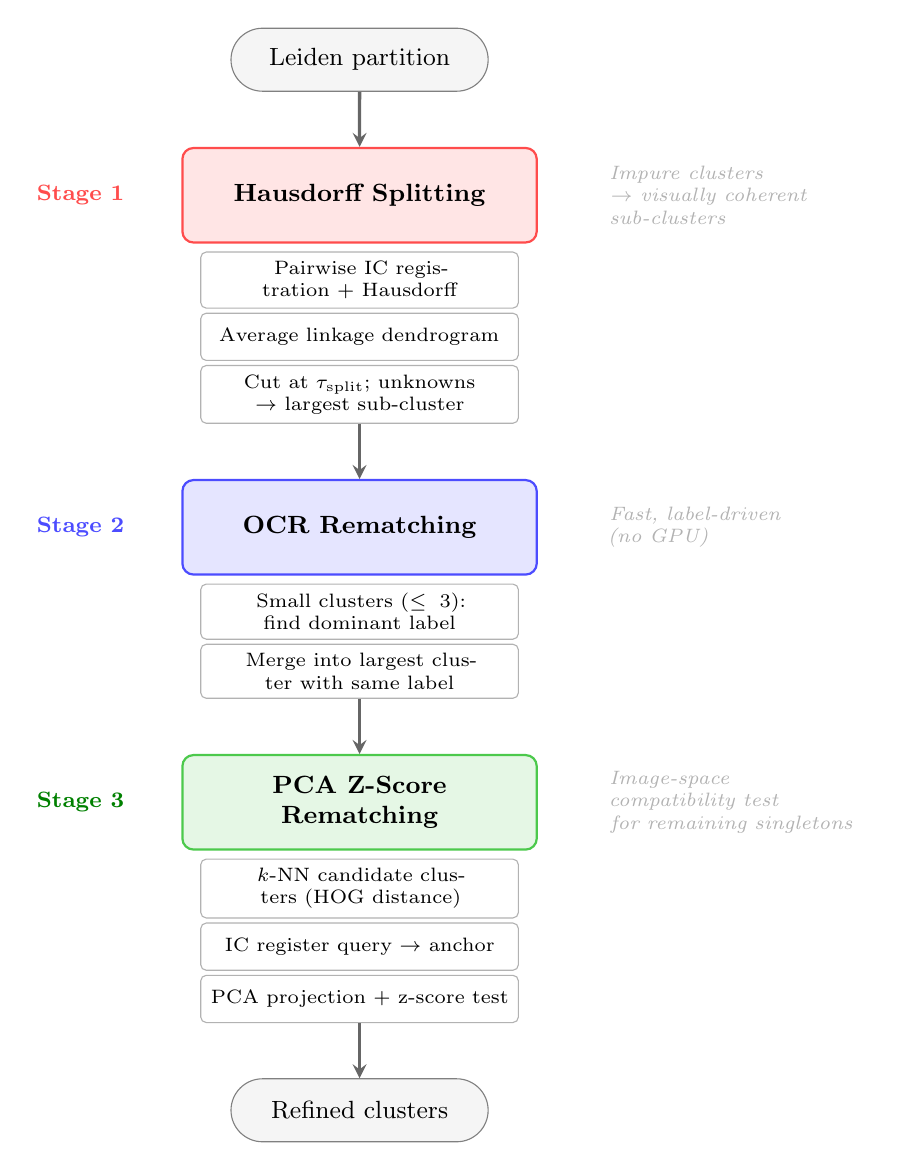
\begin{tikzpicture}[
        >=stealth,
        node distance=0.3cm and 1.5cm,
        stage/.style={
            rectangle, rounded corners=4pt, draw=#1!70, thick,
            fill=#1!10, minimum width=4.5cm, minimum height=1.2cm,
            text centered, font=\small\bfseries, text width=4.2cm
        },
        detail/.style={
            rectangle, rounded corners=2pt, draw=black!30,
            fill=white, minimum width=4.0cm, minimum height=0.6cm,
            text centered, font=\scriptsize, text width=3.8cm
        },
        io/.style={
            rounded rectangle, draw=black!50, fill=gray!8,
            minimum width=3.5cm, minimum height=0.8cm,
            text centered, font=\small
        },
        arrow/.style={->, very thick, black!60},
        note/.style={font=\scriptsize\itshape, text=gray!60, text width=3.2cm, align=left},
    ]

    % ── Input ──
    \node[io] (input) {Leiden partition};

    % ── Stage 1: Hausdorff split ──
    \node[stage=red, below=0.7cm of input] (split) {Hausdorff Splitting};
    \node[detail, below=0.1cm of split] (split1) {Pairwise IC registration + Hausdorff};
    \node[detail, below=0.05cm of split1] (split2) {Average linkage dendrogram};
    \node[detail, below=0.05cm of split2] (split3) {Cut at $\tau_\text{split}$; unknowns $\to$ largest sub-cluster};

    \node[note, right=0.8cm of split] {Impure clusters\\$\to$ visually coherent\\sub-clusters};

    % ── Stage 2: OCR rematch ──
    \node[stage=blue, below=0.7cm of split3] (ocr) {OCR Rematching};
    \node[detail, below=0.1cm of ocr] (ocr1) {Small clusters ($\le 3$): find dominant label};
    \node[detail, below=0.05cm of ocr1] (ocr2) {Merge into largest cluster with same label};

    \node[note, right=0.8cm of ocr] {Fast, label-driven\\(no GPU)};

    % ── Stage 3: PCA rematch ──
    \node[stage=green!70!black, below=0.7cm of ocr2] (pca) {PCA Z-Score Rematching};
    \node[detail, below=0.1cm of pca] (pca1) {$k$-NN candidate clusters (HOG distance)};
    \node[detail, below=0.05cm of pca1] (pca2) {IC register query $\to$ anchor};
    \node[detail, below=0.05cm of pca2] (pca3) {PCA projection + z-score test};

    \node[note, right=0.8cm of pca] {Image-space\\compatibility test\\for remaining singletons};

    % ── Output ──
    \node[io, below=0.7cm of pca3] (output) {Refined clusters};

    % ── Arrows ──
    \draw[arrow] (input) -- (split);
    \draw[arrow] (split3.south) -- ++(0,-0.2) -| ([xshift=0cm]ocr.north);
    \draw[arrow] (ocr2.south) -- ++(0,-0.2) -| ([xshift=0cm]pca.north);
    \draw[arrow] (pca3.south) -- ++(0,-0.2) -| ([xshift=0cm]output.north);

    % ── Stage labels ──
    \node[left=0.6cm of split, font=\footnotesize\bfseries, text=red!70] {Stage 1};
    \node[left=0.6cm of ocr, font=\footnotesize\bfseries, text=blue!70] {Stage 2};
    \node[left=0.6cm of pca, font=\footnotesize\bfseries, text=green!50!black] {Stage 3};

    \end{tikzpicture}%
    }
    \caption{Three-stage cluster refinement pipeline.
    After the initial Leiden partition, clusters are sequentially split by visual dissimilarity (Stage~1), merged by OCR label (Stage~2), and merged by image-space PCA compatibility (Stage~3).
    Each stage is composable and produces structured diagnostics for reporting.}
    \label{fig:refinement-pipeline}
\end{figure}


% ── Glossary construction ──
\paragraph{Glossary construction.}
The final output of the pipeline is a \emph{character glossary}: for each OCR-predicted character, we identify the cluster containing the most occurrences and select its most central member (by degree centrality in the NFA similarity graph) as the representative.
When two clusters contain equally many instances of a character, we use the mean intra-cluster NFA as a tie-breaker, selecting the cluster with the lowest mean dissimilarity (highest total NFA).
The glossary records the dominant OCR label, cluster size, and representative patch index, sorted by frequency.
This produces an inventory of all distinct character forms in the book along with their vectorised outlines.

% ── Reverse printing ──
\paragraph{Reverse printing.}
Given the glossary, the pipeline can reconstruct any page as a vector document.
For each character detection on a page, the glossary representative of its cluster is looked up and its vectorised SVG outline is rendered at the corresponding bounding-box position and scale.
The resulting overlay places clean vector outlines at the original character positions, producing a faithful reconstruction of the full page layout from the recovered character models.


% ============================================================================
%  References
% ============================================================================
\bibliographystyle{plain}
% \bibliography{references}  % uncomment when references.bib is available

% ── Inline references for standalone compilation ──
\begin{thebibliography}{99}

\bibitem{baek2019character}
Y.~Baek, B.~Lee, D.~Han, S.~Yun, and H.~Lee.
\newblock Character region awareness for text detection.
\newblock In \emph{Proc.\ IEEE/CVF CVPR}, pp.~9365--9374, 2019.

\bibitem{dalal2005histograms}
N.~Dalal and B.~Triggs.
\newblock Histograms of oriented gradients for human detection.
\newblock In \emph{Proc.\ IEEE CVPR}, vol.~1, pp.~886--893, 2005.

\bibitem{desolneux2000meaningful}
A.~Desolneux, L.~Moisan, and J.-M.~Morel.
\newblock Meaningful alignments.
\newblock \emph{Int.\ J.\ Comput.\ Vis.}, 40(1):7--23, 2000.

\bibitem{briand2018ipol}
T.~Briand, G.~Facciolo, and J.~S\'anchez.
\newblock A detailed study of the modified inverse compositional algorithm.
\newblock \emph{Image Processing On Line (IPOL)}, 8:311--364, 2018.

\bibitem{traag2019louvain}
V.~A.~Traag, L.~Waltman, and N.~J.~van Eck.
\newblock From {Louvain} to {Leiden}: guaranteeing well-connected communities.
\newblock \emph{Scientific Reports}, 9(1):5233, 2019.

\bibitem{von2010lsd}
R.~Grompone~von Gioi, J.~Jakubowicz, J.-M.~Morel, and G.~Randall.
\newblock {LSD}: a line segment detector.
\newblock \emph{Image Processing On Line (IPOL)}, 2:35--55, 2012.

\bibitem{kiessling2019kraken}
B.~Kiessling.
\newblock Kraken --- an universal text recognizer for the humanities.
\newblock In \emph{Proc.\ Digital Humanities}, 2019.

\bibitem{hubert1985comparing}
L.~Hubert and P.~Arabie.
\newblock Comparing partitions.
\newblock \emph{J.\ Classification}, 2(1):193--218, 1985.

\bibitem{rosenberg2007v}
A.~Rosenberg and J.~Hirschberg.
\newblock V-measure: A conditional entropy-based external cluster evaluation measure.
\newblock In \emph{Proc.\ EMNLP-CoNLL}, pp.~410--420, 2007.

\bibitem{rony2025hausdorff}
J.~Rony and H.~Kervadec.
\newblock Distorch: fast differentiable boundary distances.
\newblock In \emph{Proc.\ MIDL}, 2025.

\end{thebibliography}

\end{document}
